\section{Results}
\label{sec:results}

All 25 cells are solved by our criterion (in-distribution accuracy $\ge 0.95$;
the minimum observed is $0.998$), so every comparison below is between models
that learned the task.

\begin{table}[t]
\centering
\small
\caption{Extrapolation score ES (mean exact-match accuracy over $L\in\{10,12,16,20\}$),
averaged over seeds and restricted to solved runs. Best per row in bold. Two
length-coupled tasks are marked $^{\dagger}$. Every cell using an explicit
additive or rotary code sits at $0.00$; only ALiBi on copy departs from the
pattern.}
\label{tab:main}
\begin{tabular}{@{}lccccc@{}}
\toprule
Task & \nope{} & learned & sin & RoPE & ALiBi \\
\midrule
copy                    & \textbf{0.34} & 0.00 & 0.00 & 0.00 & 0.31 \\
prefix-XOR              & \textbf{0.00} & 0.00 & 0.00 & 0.00 & 0.00 \\
sort                    & \textbf{0.76} & 0.00 & 0.00 & 0.00 & 0.00 \\
swap-halves$^{\dagger}$ & 0.00 & 0.00 & 0.00 & 0.00 & 0.00 \\
reverse$^{\dagger}$     & \textbf{0.29} & 0.00 & 0.00 & 0.00 & 0.00 \\
\bottomrule
\end{tabular}
\end{table}

\paragraph{The cliff is not specific to one task.} \figref{fig:curves} repeats the
pattern of \figref{fig:padded} across the battery. With a learned, sinusoidal or
rotary code, accuracy is $1.00$ at the training length and $0.00$ at the next one
tested, on every task where the task can be learned at all. \nope{} instead decays
smoothly where the task permits extrapolation (copy $0.96$ at $L{=}10$, reverse
$0.87$, sort $1.00$). Twenty-one of the twenty-five cells have ES below $0.01$,
eighteen exactly zero; the discrimination between methods comes from the four
cells that clear it.

\paragraph{The failure is not an out-of-distribution position.} The standard
format cannot distinguish the two accounts, since $2L+1$ positions grow with $L$.
\figref{fig:padded} removes the confound: every example is padded to a fixed 41
tokens with the separator pinned at index 21, so all positions occur in training
and only the effective length varies. Under this protocol the learned and
sinusoidal codes still fall from $1.00$ at $L{=}8$ to $0.00$ at $L{=}10$, whereas
\nope{} retains $0.79$ and ALiBi $0.87$, decaying to $0.02$ and $0.10$ at
$L{=}12$. Padding costs some accuracy overall---\nope{} reaches $0.96$ at $L{=}10$
in the standard format and $0.79$ here, plausibly because half the sequence is
now filler---but the ordering is unchanged and the collapse is undiminished. With
no unseen position left to blame, the failure has to be indexed by length.

\begin{figure}[t]
\centering
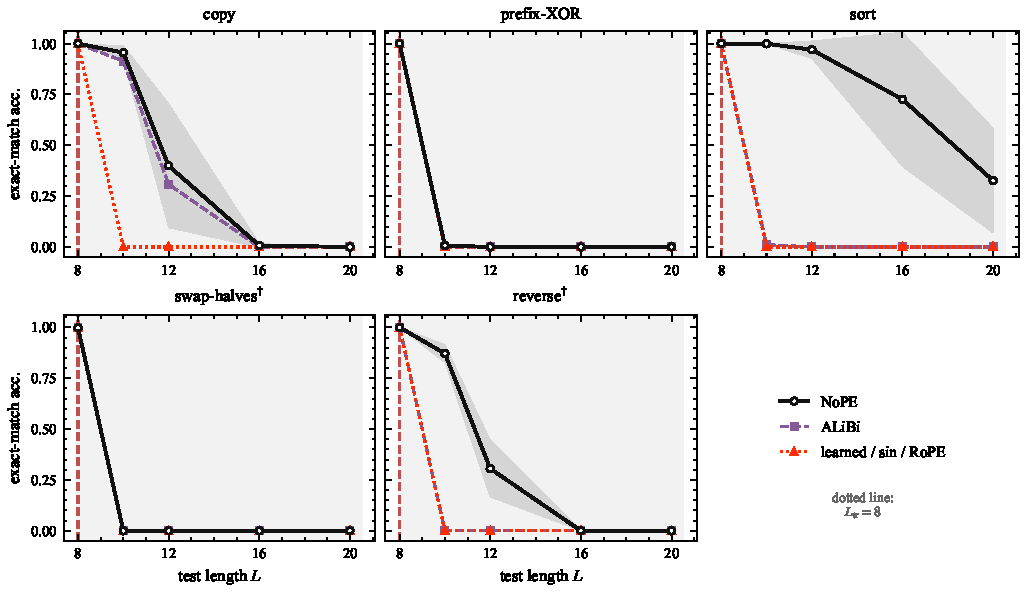
\includegraphics[width=\textwidth]{../figures/fig1_curves.pdf}
\caption{Exact-match accuracy versus test length, one panel per task, mean over
seeds with $\pm$1 s.d. The dotted line marks the training length. Learned,
sinusoidal and rotary codes coincide numerically, so they are drawn as one curve;
all three fall to zero at the first length beyond training. \nope{} instead
decays gradually on the three tasks it can extrapolate at all, and fails on the
remaining two. Tasks are ordered by length-coupling, coupled ones marked $*$.}
\label{fig:curves}
\end{figure}

\paragraph{A task-side explanation does not fit.} Before settling on the lookup
account we tested the most natural alternative: that the effect is organised by
whether a task's positional rule is written in terms of $L$ (\secref{sec:method}).
Under that account the ranking of encodings should reverse between classes, with
\nope{} losing its advantage on the coupled tasks. It does not. \nope{} is at or
near the top of every task, and the spread between the best and worst encoding is
$0.34$ (copy), $0.76$ (sort) and $0.29$ (reverse)---larger on the decoupled side
($0.37$ mean) than the coupled side ($0.15$). What the data do show is that
heterogeneity is real: a two-way ANOVA treating seed as a replicate ($n{=}50$)
gives a task$\times$encoding interaction of $F(16,25)=32.3$, $p<10^{-3}$,
$\eta_p^2=0.95$. Encodings do behave differently across tasks; the difference is
just not organised by coupling. We report this because it cuts against the
explanation we set out to test, and because a null interaction would have been a
weaker finding. The test treats seeds as independent replicates, an approximation
that if anything understates the residual variance.

\paragraph{Where every method fails, the obstacle is not positional.} On
prefix-XOR and swap-halves, \emph{every} condition including \nope{} scores at or
below $0.01$ despite reaching $\ge 0.998$ in-distribution. The obstacle there is
the difficulty of representing the underlying algorithm in a length-invariant way,
the phenomenon studied by \citet{zhou2023what}, and no choice of positional
encoding can address it. Keeping these tasks in the battery is what makes that
visible: it bounds what any PE intervention could achieve.
